\documentclass[11pt]{article}

\usepackage{lastpage}
\usepackage{afterpage}
\usepackage{boxedminipage}
\usepackage{enumerate}
\usepackage{fullpage}
\usepackage{graphicx}

%%--------------------------------------------------------------------
%%
%%        Pages

\newcommand{\totalquestions}{{\bf XXX}}
\newcommand{\totalpages}{\pageref{LastPage}}
\setlength{\parskip}{4pt}
\setlength{\parindent}{0cm}
%\renewcommand{\thepage}{Page \arabic{page} of \totalpages}

%%--------------------------------------------------------------------
%%
%%        Textwidth

\newlength{\subtextwidth}
\setlength{\subtextwidth}{\textwidth}
\addtolength{\subtextwidth}{-2ex}
\newcommand{\fullwidthbox}[1]{\framebox[\textwidth]{\parbox{\subtextwidth}{#1}}}

%%--------------------------------------------------------------------
%%
%%        Counting Parts

\newcounter{epart}
\newcommand{\epart}[1]{%[2]{
    \stepcounter{epart}
    \section*{Part \Alph{epart}~--~#1} %\hfill
            %{\large [{#1} marks, {#2} mins]}}
  }

%%--------------------------------------------------------------------
%%
%%        Counting questions

\newcounter{question}
\newcommand{\question}[1]{
    \stepcounter{question}
    \subsection*{Question \thequestion \hfill
      {\normalsize [{#1}]}} }


%%--------------------------------------------------------------------
%%
%%        The Exam!


\begin{document}
%%
%%--------------------------------------------------------------------
%%
%%        The University Crest
%%
\vspace{5ex}
\begin{center}
\textbf{\sc The University of Melbourne}\\[0.5ex]
\textbf{\sc COMP90020: Distributed Algorithms}\\[1ex]
\textbf{\large Question Pool, SM1 2021}\\
\end{center}

\newpage


%Clock Synchronization
\section {Clock Synchronization}

\question{Exam18/19} 
Consider two asynchronous distributed systems $AS_1$ and $AS_2$. Cristian's algorithm is used in both systems to synchronize clocks. In $AS_1$, the minimum transmission delay $T_{min}$ is estimated to be 0.3 seconds and process $p_1$ records a round trip time $T_{round}$ of 1.6 seconds. In $AS_2$, $T_{min}$ is estimated to be 1.2 seconds and $p_2$ records a round trip time of 2.8 seconds. Which process can achieve a higher accuracy? Explain your answer.

\question{new} 
If we know that event $a$ happened before event $b$ in absolute physical time, will either the Berkeley algorithm or Cristian's algorithm guarantee that the timestamp of $a$ is less than the timestamp for $b$? Explain your answer.

\question{new}
Cristian's clock synchronization algorithm assumes symmetric message transmission delays; that is, the transmission delay of the request message ($m_r$) is expected to be the same as the transmission delay of the response message ($m_t$). This is not true in all networks. How would you modify the formula for setting a process's clock ($C_p$) if the transmission delay of the request message is 3 times longer than the transmission delay of the response message? Show your calculations and notations clearly.

\question{new}
Cristian's clock synchronization algorithm assumes symmetric message transmission delays; that is, the transmission delay of the request message is expected to be the same as the transmission delay of the response message. This is not true in all networks.
\begin{enumerate}
	\item Reformulate the algorithm to accommodate asymmetric delays, where $C_s$ is the server's time, $T_{m_r}$ is the time the request was sent, $T_{m_t}$ is the time the response was received, $B_u$ is the upstream bandwidth from the process to the server, $B_d$ is the downstream bandwidth form the server to the process. Assume all messages are of size $M$.
	\item Assume a network with X downstream bandwidth and X upstream bandwidth. A process makes a request at time X and gets a response X msec later. If the time on the server is X, what would the process set its clock to?  [change X for actual values]
\end{enumerate}

\question{new} 
A process's clock reads X. The server's clock reads Y when they synchronize using the Berkeley algorithm. Assume message delays are negligible. What does the process sets its clock to after synchronization?


\question{new} 
A client's clock reads X. The server's clock reads Y when they synchronize using Cristian's algorithm. Assume message delays are negligible.  What does the process sets its clock to after synchronization?

\question{Sample19 4}
Using Cristian's method for synchronizing clocks where we use a time server, we record the  round-trip  time  and  the  timestamp  returned  by  the  server  as  4  sec  and  9:55:28,  respectively.  What  time  should  we  set  the  local  clock  to?  What  is  the  accuracy  of  this  setting? What is the accuracy of the setting if we know for a fact that minimum round trip time is 1 sec. Show your calculations and notation clearly.

\section{Logical Time}

\question{new}
Assign Lamport timestamps to the following events: [give diagram with events and some timestamps]

\question{new}
Assign Vector timestamps to the following events: [give diagram with events and some timestamps]

\question{new}
Which set of events is concurrent? [multiple choice, give sets of 2 or 3 vector timestamps]

\question{Exam18/19 4}
Assume we have three processes: $p_{1}$, $p_{2}$ and $p_{3}$. Each process can only communicate with another single process (multicasting or broadcasting is not allowed). Is it possible to construct a sequence of events that only consists of send events (denoted as $s_{i}$) and receive events (denoted as $r_{i}$) such that all three processes are concurrent and all have Lamport clock values that are equal to 3? Note that we assume that every process has to send and receive at least one message. If your answer is yes, provide an example sequence for all 3 processes. If your answer is no, explain why.

\section{Global Sates and Snapshots}


\question{new}
examples of linearization, consistent/inconsistent cut, etc.

\question{Exam18 4}
Do we have to assume in the Chandy-Lamport snapshot algorithm that all channels are FIFO to ensure that the recorded global state is consistent? Explain your answer. 

\question{new}
In the Chandy-Lamport snapshot algorithm, the marker sending rule states that after recording its state, a process must send a marker on every outgoing channel before sending out any other messages.
 
 \begin{itemize}
 	\item (option a) Explain the importance of this rule. To help your answer, illustrate with an example what would happen if after recording its state, a process was allowed to send application messages before sending out the marker. 
 	\item (option b) Explain why the marker must be sent before any other messages. Give an example to illustrate your answer. 
 \end{itemize}
 
\question{Exam19 2}
Is it true that in a consistent snapshot, all the recorded local states of processes are concurrent? Explain your answer.

\section{Mutual Exclusion}

\question{Exam18/19 4}
Is the following statement true? In the Ricart-Agrawala algorithm, the critical section is accessed according to the order of increasing timestamps. Explain your answer.

\question{Exam19 3}
Explain in detail how Maekawa's voting algorithm ensures the safety condition.

\question{new}
maekawa and voting sets, what would happen if one of the conditions was not met...

\question{new}
maekawa and deadlocks

\question{Book}
Give an example execution of the ring-based algorithm to show that processes are not necessarily granted entry to the critical section in happened-before order.

\question{Book}
In a certain system, each process typically uses a critical section many times before another process requires it. Explain why Ricart and Agrawala?s multicast-based mutual exclusion algorithm is inefficient for this case, and describe how to improve its performance. Does your adaptation satisfy liveness condition ME2?

\question{new}
Assume the Bully algorithm as seen in the lectures is implemented in an asynchronous distributed system. Discuss the implications of doing this in terms of safety. Use an example to illustrate your answer. 

\question{Exam18 4}
The Bully algorithm is not guaranteed to meet the safety condition. The algorithm assumes that each process's failure detector is reliable. Which condition, safety or liveness, may not be guaranteed if a failure detector is unreliable? Explain what could happen for an unreliable failure detector.

\question{new}
Suppose the Ricart and Agrawala's algorithm for mutual exclusion is implemented incorrectly -- instead of labeling requests with <$T_i$,  $P_i$> it labels them with <$P_i$,  $T_i$>. The rest of the algorithm is unchanged. Does this algorithm still satisfy safety, liveness, and ordering? Explain your answer.  

\question{Exam18/19 4}
Is the following statement true? in the Ricart-Agrawala algorithm, the critical section is accessed according to the order of increasing timestamps. Explain your answer.

\question{new}
maekawa and voting sets, what would happen if one of the conditions was not met


%Leader Election


\question{new}
Consider a synchronous distributed system with 5 processes, $p_1$, $p_2$, $p_3$, $p_4$, and $p_5$. $p_5$ is currently the coordinator and when $p_5$ crashes, it is $p_2$ that notices the coordinator is down. Suppose the Bully algorithm is used to elect a new coordinator by choosing the process with the largest identifier (i.e., $p_1 < p_2 < p_3 < p_4 < p_5$). Assume there are no failures in the system during the election run. Show the set of all messages that are sent during the election run. Clearly indicate for each message the sending process, the receiving process, and the type of message (i.e., election, coordinator, or answer).

\question{new}
Discuss the limitations of using an unreliable failure detector to enable the ring-based leader election algorithm seen in the lectures to tolerate crash failures. Consider two cases in your answer, i) the process with the highest ID in the system crashes during an election run, ii) a process with an ID that is not the highest ID in the system crashes during an election run.

\question{new}
Consider a distributed system with 5 processes arranged in a logical ring with unidirectional clockwise communication links as shown in Figure \ref{worstcaseRBEFig}. 

Considering the ring-based leader election algorithm we discussed in the lectures, what would the bandwidth consumption be (i.e., the number of exchanged messages) if all 5  processes initiated an election at the same time? Explain your answer.

What would the bandwidth consumption be if the ring was arranged as shown in Figure \ref{bestcaseRBEFig} and all 5 processes initiated an election at the same time? Explain your answer.

\question {new}
number of messages in ring-based election when every process initiates the algorithm, students to identify best and worst cases (see question above).

\question{Sample19 4}
Explain,  briefly,  what  happens  if  two  processes  simultaneously  start  elections  using  the  ring-based election algorithm that we saw in class. Is this a problem for the algorithm? 

\question{new}
 Consider the ring-based election algorithm we saw in class. Explain why participating processes can safely suppress (i.e., do not forward) election messages that contain IDs smaller than their own. Explain what would happen if the algorithm did not have this rule in place and i) multiple processes initiated an election simultaneously, ii) a single process initiated an election.
 
 \question{new}
 \begin{itemize}
 	\item
 	Version 1. Consider the ring-based election algorithm we saw in class. Explain in which situation would a participating process receive an election message with an ID smaller than its own. Explain why participating processes can safely suppress (i.e., do not forward) election messages that contain IDs smaller than their own. Explain what would happen if the algorithm did not have this rule in place. 
 	
 	\item
 	Version 2. Consider the ring-based election algorithm we saw in class. Explain why participating processes can safely suppress (i.e., do not forward) election messages that contain IDs smaller than their own. Explain what would happen if the algorithm did not have this rule in place and i) multiple processes initiated an election simultaneously, ii) a single process initiated a single election.
 	
 \end{itemize}

\question{new}
Assume the Bully algorithm as seen in the lectures is implemented in an asynchronous distributed system. Discuss the implications of doing this in terms of safety. Use an example to illustrate your answer. 

(or...discuss safety in the bully algorithm if T is not accurate, give examples)

\question{new}
Discuss the limitations of using an unreliable failure detector to enable the ring-based leader election algorithm seen in the lectures to tolerate crash failures. Consider two cases in your answer, i) the process with the highest ID in the system crashes during an election run, ii) a process with an ID that is not the highest ID in the system crashes during an election run.


\section{Multicast}

\question{Book 4}
Suggest how to adapt the causally ordered multicast protocol to handle overlapping groups.

 \question{Sample19 4}
The figure below (Figure \ref{orderedMulticastFig}) shows some multicast messages happening for three processes on different machines. Is the ordering of these multicast messages CO, FIFO and/or TO? Explain your answer.

\begin{figure}[h]
	\includegraphics[scale=0.6]{orderedMulticast}
	\caption{Ordered multicast example}
	\label{orderedMulticastFig}
\end{figure}

\question{Exam19 3}
Name all properties of a TO (totally ordered) reliable  multicast.

\question{Exam18/19 4}
Assume we implement causal ordering using vector timestamps for processes that belong to group $g$. If process $p_3$ receives a message $< m,V^2_g = [4,6,2] >$ from process $p_2$ at vector timestamp $V3g = [3, 5, 2]$, can $p_3$ B-deliver the message? Explain your answer.

\question{new}
Is the following statement true or false for the implementation of reliable multicast using basic multicast seen in the lectures:

If a process multicasts a message to a group, either all processes in the group deliver the message, or none do.

Justify your answer. If it is true, show why. If it is false, show a counterexample. 

\question{new}
Consider a distributed system that connects every pair of processes through a communication channel. Channels are reliable and guarantee that messages arrive in FIFO order. Assume processes do not fail and that a process delivers a message to itself before sending it out to any other process. 

\begin{enumerate}
	\item If B-multicast was used in this system, would FIFO, causal, and/or total ordering be guaranteed? Justify your answer by explaining why an ordering is guaranteed, or by presenting an example that demonstrates why it is not.
	\item If R-multicast was used in this system, would FIFO, causal, and/or total ordering be guaranteed? Justify your answer by explaining why an ordering is guaranteed, or by presenting an example that demonstrates why it is not.
\end{enumerate}

\question{new}
Consider a distributed system with 2 processes, $p_1$ and $p_2$, connected through a communication channel. The channel is reliable and guarantees that messages arrive in FIFO order. Assume processes do not fail and that a process delivers a message to itself before sending it out to any other process. If B-multicast was used in this system, would FIFO, causal, and/or total ordering be guaranteed? Justify your answer by explaining why an ordering is guaranteed, or by presenting an example that demonstrates why it is not.

\question{Sample19 4}

In  the  following  reliable  multicast  algorithm (Figure \ref{rmulticastFig}) that  we  saw  in  class,  explain  briefly  what  would happen if we were to have `R-deliver m' before the `if (q $\neq$ p) then...' statement.

\begin{figure}[h]
	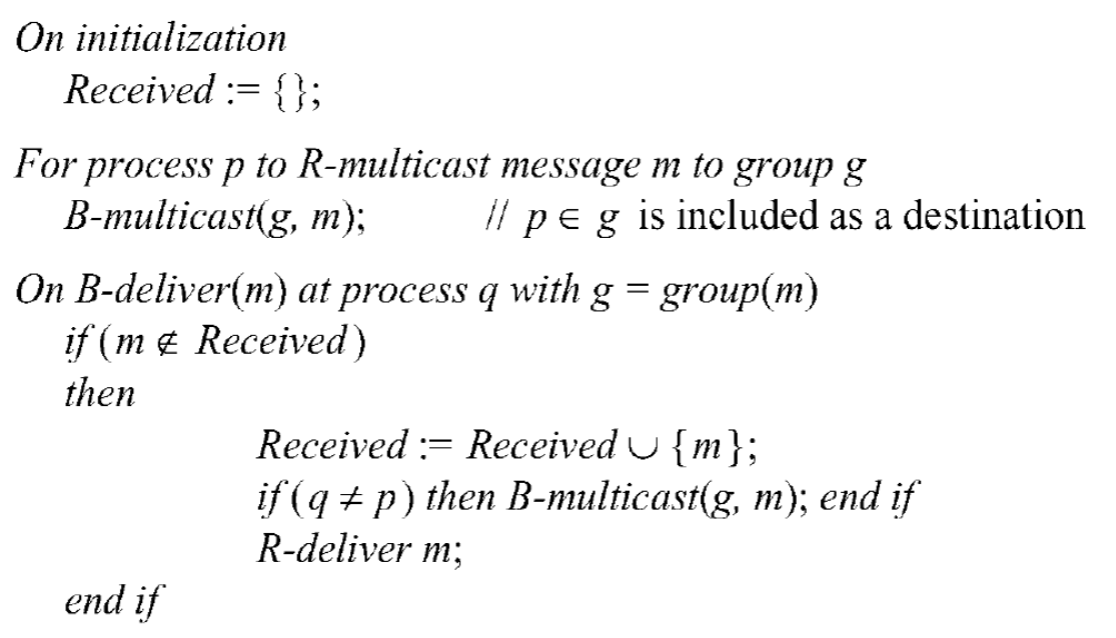
\includegraphics[scale=0.6]{rmulticast}
	\caption{Reliable multicast algorithm}
	\label{rmulticastFig}
\end{figure}

\question{new}
total causal, or total fifo ordering

\question{new}
ordered multicast for more than one group

\question{new}
show that causal does not imply total, show that total does not imply causal, show that fifo does not imply causal, show that causal implies fifo






\end{document}
